\documentclass{article}

\usepackage{geometry}
\usepackage{amsmath}
\usepackage{graphicx, eso-pic}
\usepackage{listings}
\usepackage{hyperref}
\usepackage{multicol}
\usepackage{fancyhdr}
\pagestyle{fancy}
\fancyhf{}
\hypersetup{ colorlinks=true, linkcolor=black, filecolor=magenta, urlcolor=cyan}
\geometry{ a4paper, total={170mm,257mm}, top=10mm, right=20mm, bottom=20mm, left=20mm}
\setlength{\parindent}{0pt}
\setlength{\parskip}{0.3em}
\renewcommand{\headrulewidth}{0pt}

\rfoot{\thepage}
\fancyhf{} % sets both header and footer to nothing
\renewcommand{\headrulewidth}{0pt}
\lfoot{\textbf{CnC Intern Contest}}
\pagenumbering{gobble}

\fancyfoot[CE,CO]{\thepage}
\lstset{
    basicstyle=\ttfamily\small,
    columns=fixed,
    extendedchars=true,
    breaklines=true,
    tabsize=2,
    prebreak=\raisebox{0ex}[0ex][0ex]{\ensuremath{\hookleftarrow}},
    frame=none,
    showtabs=false,
    showspaces=false,
    showstringspaces=false,
    prebreak={},
    keywordstyle=\color[rgb]{0.627,0.126,0.941},
    commentstyle=\color[rgb]{0.133,0.545,0.133},
    stringstyle=\color[rgb]{01,0,0},
    captionpos=t,
    escapeinside={(\%}{\%)}
}

\begin{document}

\begin{center}

    
    \section*{Ambiguitas Kota} % ganti judul soal

    \begin{tabular}{ | c c | }
        \hline
        Batas Waktu  & 1s \\    % jangan lupa ganti time limit
        Batas Memori & 256MB \\  % jangan lupa ganti memory limit
        \hline
    \end{tabular}
\end{center}

\subsection*{Deskripsi}
Terdapat sebuah negara dengan $N$ buah kota dan $M$ buah jalan. Negara ini memiliki sebuah Ibukota. Setiap jalan di negara ini hanya memiliki 1 arah dan juga memiliki jarak. Sepasang kota A dan B dikatakan ambigu apabila jarak antara kota A dengan Ibukota negara tersebut sama dengan jarak antara kota B dengan Ibukota negara tersebut. Cari jumlah pasangan ambigu di negara tersebut!. 

\subsection*{Format Masukan}
Baris pertama terdiri dari tiga bilangan bulat positif yaitu $N$ ($1 \leq N \leq 1.000.000$) menyatakan banyaknya kota,
$M$ ($0 \leq M \leq N\times(N-1) $) yang menyatakan banyak jalan, dan $K$ ($1 \leq K \leq N$) yang menyatakan nomor kota yang dijadikan sebagai Ibukota

$M$ baris selanjutnya terdiri atas 3 bilangan bulat positif yaitu $U$ ($1 \leq U \leq N$), $V$ ($1 \leq V \leq N$), dan $W$ ($1 \leq W \leq 10^9$) yang menyatakan bahwa terdapat jalan antara kota $U$ dan kota $V$ dengan panjang jalan tersebut adalah $W$

Dipastikan bahwa antara Kota $U$ ke kota $V$ akan ada hanya 1 jalan. Akan tetapi, tidak menutup kemungkinan bahwa akan ada jalan dari kota $V$ ke kota $U$.
Dipastikan juga bahwa tidak ada jalan yang dimulai dan berakhir di kota yang sama
\subsection*{Format Keluaran}
Keluarkan sebuah bilangan bulat yang menyatakan jumlah pasangan kota ambigu dalam negara tersebut!

\\

\begin{multicols}{2}
\subsection*{Contoh Masukan}
\begin{lstlisting}
7 6 4
4 5 1
4 1 1
5 6 2
1 2 2
6 2 10
1 3 10

\end{lstlisting}
\columnbreak
\subsection*{Contoh Keluaran}
\begin{lstlisting}
2 
\end{lstlisting}
\vfill
\null
\end{multicols}


\pagebreak
\subsection*{Penjelasan}
\begin{center}
    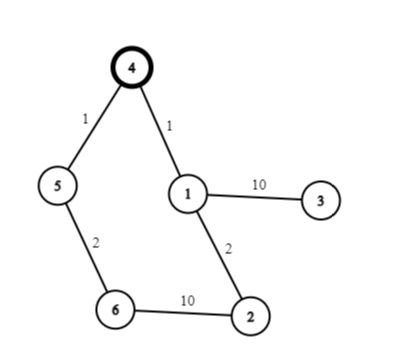
\includegraphics{graph.png}
\end{center}
Pasangan ambigu adalah pasangan kota 5 dan kota 1 dan pasangan kota 6 dan kota 2


\pagebreak

\end{document}